% ==============================================================================
% MLSys 2026 FlashInfer-Bench Challenge — Track A Poster
% A0 Landscape, beamerposter, 4-column layout
% ==============================================================================

\documentclass[final,t]{beamer}
\usepackage[size=a0,scale=1.15,orientation=landscape]{beamerposter}
\usetheme{default}
\setbeamertemplate{navigation symbols}{}
\setbeamertemplate{itemize items}[circle]

% Packages
\usepackage{graphicx}
\usepackage{amsmath,amssymb}
\usepackage{booktabs}
\usepackage{hyperref}
\usepackage{array}
\usepackage{xcolor}

% ---- Color scheme ----
\definecolor{PosterBlue}{RGB}{0,51,102}
\definecolor{PosterLightBlue}{RGB}{228,238,250}

\setbeamercolor{block title}{bg=PosterBlue,fg=white}
\setbeamercolor{block body}{bg=PosterLightBlue,fg=black}
\setbeamercolor{block alerted title}{bg=PosterBlue,fg=white}
\setbeamercolor{block alerted body}{bg=PosterLightBlue,fg=black}

% ---- Fonts ----
\setbeamerfont{block title}{size=\Large,series=\bfseries}
\setbeamerfont{block body}{size=\normalsize}

% Compact block spacing (no extra gaps between blocks)
% Helper macros to hide split begin/end from linter
\makeatletter
\newcommand{\opencolorbox}[2]{\@nameuse{beamercolorbox}[#1]{#2}}
\newcommand{\closecolorbox}{\@nameuse{endbeamercolorbox}}
\makeatother
\setbeamertemplate{block begin}{
  \vskip0.2ex
  \opencolorbox{colsep*=0.5ex}{block title}%
    \usebeamerfont*{block title}\insertblocktitle
  \closecolorbox%
  {\nointerlineskip\vskip-0.5pt}%
  \usebeamerfont{block body}%
  \opencolorbox{colsep*=0.5ex,vmode}{block body}%
}
\setbeamertemplate{block end}{
  \closecolorbox\vskip0.2ex
}
\setbeamertemplate{block alerted begin}{
  \vskip0.2ex
  \opencolorbox{colsep*=0.5ex}{block alerted title}%
    \usebeamerfont*{block title}\insertblocktitle
  \closecolorbox%
  {\nointerlineskip\vskip-0.5pt}%
  \usebeamerfont{block body}%
  \opencolorbox{colsep*=0.5ex,vmode}{block alerted body}%
}
\setbeamertemplate{block alerted end}{
  \closecolorbox\vskip0.2ex
}

\setbeamersize{text margin left=10mm, text margin right=10mm}

% Column gap
\newlength{\colsep}
\setlength{\colsep}{8mm}

% Fixed column height (A0 landscape height minus header, footer, margins)
\newlength{\colheight}
\setlength{\colheight}{729mm}

% ==============================================================================
\begin{document}
\begin{frame}[t]

% ---- HEADER ----
\begin{beamercolorbox}[wd=\textwidth,sep=0.4cm]{block title}
\centering
{\VeryHuge\bfseries\color{white}Fused MoE Inference on Blackwell:\\[0.1cm]A Workload-Adaptive Kernel System for DeepSeek-V3}\\[0.25cm]
{\LARGE\color{white}Jiayao Zhang \quad Jiaoliang Yu \qquad {\color{PosterLightBlue}MLSys 2026 FlashInfer-Bench Challenge --- Track A}}
\end{beamercolorbox}

\vspace{0.05cm}

% ---- MAIN CONTENT (minipage-based for explicit gap control) ----
\noindent
\begin{minipage}[t]{0.225\textwidth}
\begin{minipage}[t][\colheight][t]{\textwidth}

\begin{block}{Motivation}
\begin{itemize}
\item DeepSeek-V3 MoE: 256 routed experts (32 local per GPU), top-8 routing, $H{=}7168$, $I{=}2048$; two FP8 block-scaled GEMMs per forward pass
\item \textbf{Hardware:} NVIDIA B200 (Blackwell, sm\_100a) --- ${\sim}2{,}500$ TFLOPS FP8, 96\,MB L2, 8\,TB/s HBM3e
\item Na\"ive per-expert loop: kernel launch overhead dominates small $T$; atomic scatter hurts large $T$
\item \textbf{Goal:} Workload-adaptive fused kernel system covering $T{=}1$ to $14{,}107$ with Triton pipeline + CuTe hybrid for largest traces
\end{itemize}
\end{block}

\begin{block}{Five-Stage Pipeline}
\begin{center}
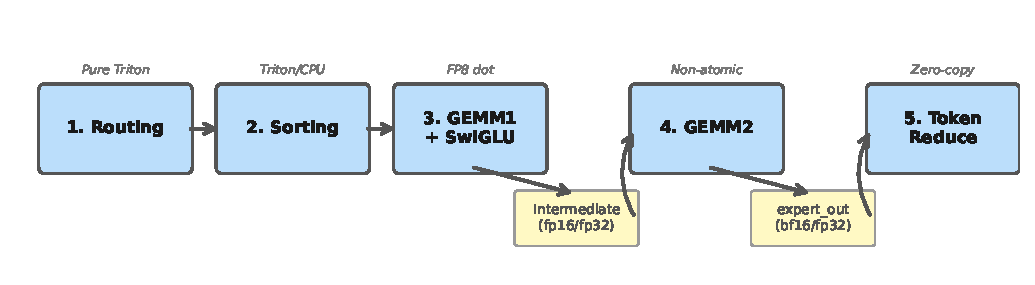
\includegraphics[width=0.95\linewidth]{figures/pipeline.pdf}
\end{center}
\begin{enumerate}
\item \textbf{Routing:} Triton DeepSeek-V3 no-aux routing (sigmoid, group top-4, global top-8, normalization)
\item \textbf{Sorting:} Tile-parallel histogram with atomic offsets and padded row construction
\item \textbf{GEMM1+SwiGLU:} Fused $W_1$/$W_3$ projections in shared K-loop with \texttt{tl.dot(fp8,fp8)}
\item \textbf{GEMM2:} Non-atomic down-projection $\to$ \texttt{expert\_out} (bf16)
\item \textbf{Token Reduce:} 2D tiled accumulation of $K{=}8$ expert contributions per output token
\end{enumerate}
Singleton $T{=}1$ and large-$T$ CuTe paths reuse the same stages with specialized kernels.
\end{block}

\begin{block}{Experimental Setup}
\begin{itemize}
\item \textbf{HW/SW:} B200 (sm\_100a), PyTorch 2.12+cu132, Triton 3.7.0
\item \textbf{Scoring:} CUPTI GPU kernel time only; CPU overhead (routing, sorting, ${\sim}600\,\mu$s) excluded from score
\item \textbf{Tolerance:} atol=1.0, rtol=0.3, 90\% ratio --- ${\sim}100\times$ wider than our strict validation (atol=0.01)
\item \textbf{Workloads:} 19 real-trace batches ($T{=}1$ to $14{,}107$); same-session A/B testing with ${\pm}2\%$ mean noise floor
\item \textbf{Baseline:} FlashInfer reference MoE kernel (PyTorch-based per-expert dispatch)
\end{itemize}
\end{block}

\begin{block}{Workload-Adaptive Dispatch}
\small
\begin{tabular}{@{}lll@{}}
\toprule
\textbf{Regime} & \textbf{BM} & \textbf{Path} \\
\midrule
$2 \le T \le 128$ & 16 & Generic Triton \\
$129 \le T \le 512$ & 32 & Generic Triton \\
$513 \le T \le 2047$ & 64 & Generic Triton \\
$T \ge 2048$ & 128 & Generic (exact launch) \\
\midrule
$T{=}1$ & 16 & Singleton Triton \\
$T{=}53$--59 & 8 & Tight-padding Triton \\
$T{=}901$ & 64 & Isolated Triton \\
$T{=}11948,14107$ & 128 & Triton/CuTe hybrid \\
\bottomrule
\end{tabular}
\normalsize
\vspace{4pt}

$T{\ge}4096$: exact grid from \texttt{total\_blocks} avoids ${\sim}30\%$ idle blocks. CuTe handles the grouped GEMM core for the largest traces; Triton handles metadata and epilogues.
\end{block}

\end{minipage}
\end{minipage}%
\hspace{\colsep}%
\begin{minipage}[t]{0.245\textwidth}
\begin{minipage}[t][\colheight][t]{\textwidth}

\begin{block}{Key Optimizations}

{\large\bfseries 1. FP8 Native Tensor Core Dot \hfill $\boldsymbol{2\times}$ throughput}
\vspace{2pt}

\texttt{tl.dot(fp8, fp8)} on Blackwell \texttt{tcgen05.mma}; block-scale dequant \emph{after} the dot. Fused $W_1$/$W_3$ gate/up in shared K-loop with inline SwiGLU, eliminating a separate elementwise kernel.

\vspace{4pt}\rule{\linewidth}{0.3pt}\vspace{4pt}

{\large\bfseries 2. Non-Atomic GEMM2 + Token Reduce \hfill $\boldsymbol{+46\%}$}
\vspace{2pt}

Atomic scatter = $6\times$ BW amplification (12\,B FP32 RMW vs.\ 2\,B bf16 store). Two-pass design: GEMM2 writes bf16 \texttt{expert\_out} (non-atomic); separate token-reduce kernel accumulates $K{=}8$ expert contributions per token in FP32. Fused atomic alternative tested and rejected ($-4.5\%$ on large $T$).

\vspace{4pt}\rule{\linewidth}{0.3pt}\vspace{4pt}

{\large\bfseries 3. FP16 Intermediate ($\times$0.125/$\times$8.0) \hfill $\boldsymbol{+4.5\%}$}
\vspace{2pt}

SwiGLU spans ${\pm}40$K (exceeds FP16 max 65504). Scale $\times$0.125 in GEMM1 $\to$ FP16 store $\to$ $\times$8.0 in GEMM2. Halves HBM traffic on $[\text{MAX\_PADDED}, 7168]$ Intermediate. FP32 fallback for $T{<}32$.

\vspace{4pt}\rule{\linewidth}{0.3pt}\vspace{4pt}

{\large\bfseries 4. Workload-Adaptive Dispatch}
\vspace{2pt}

BLOCK\_M = 8/16/32/64/128 by token count. Column-major (GROUP\_M=32/64) for L2 reuse. $T{=}1$: fused singleton kernels. $T{=}53$--59: BLOCK\_M=8. $T{\ge}2048$: exact grid launch. Largest traces: CuTe grouped-GEMM core.

\vspace{4pt}\rule{\linewidth}{0.3pt}\vspace{4pt}

{\large\bfseries 5. Compiler Hints \& Cache Policy \hfill $\boldsymbol{+4.9\%}$}
\vspace{2pt}

Disable LLVM loop-strength-reduction (\texttt{LSR=off}) to avoid register spills on high-occupancy kernels. Asymmetric L2 cache policy: weights \texttt{evict\_last} (reused across M-tiles), tokens \texttt{evict\_first} (streamed once).

\vspace{4pt}\rule{\linewidth}{0.3pt}\vspace{4pt}

{\large\bfseries 6. Deep Pipeline + 2D Reduce \hfill $\boldsymbol{+5\%}$}
\vspace{2pt}

GEMM2 \texttt{num\_stages=6--8} hides HBM latency (+2.1\%). 2D tiled reduce (BLOCK\_M$\times$BLOCK\_N) cuts grid $>$10$\times$ vs.\ 1D row-per-CTA (+2.9\% large-$T$).

\end{block}

\begin{block}{Precision Hierarchy}
\begin{center}
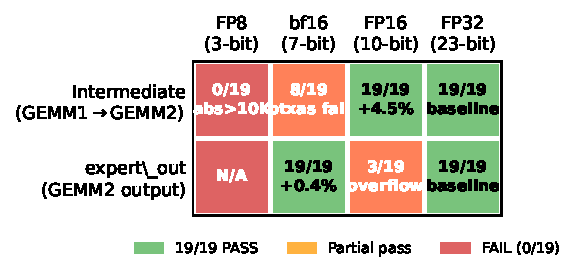
\includegraphics[width=0.85\linewidth]{figures/precision_matrix.pdf}
\end{center}
\textbf{Intermediate} (GEMM1$\to$GEMM2): requires $\ge$FP16. SwiGLU spans ${\pm}40$K (fp8 max = 448); bf16 passes 8/19 only. Scaling $\times$0.125/$\times$8.0 clamps to FP16-safe range, halving HBM traffic.

\textbf{Expert output} (GEMM2$\to$reduce): bf16 OK (range $3.4{\times}10^{38}$); fp16 overflows 3/19. bf16 saves 50\% write BW (+0.4\%). Contest $\text{atol}{=}1.0$ accommodates bf16 precision loss.

\textbf{MXFP8} (\texttt{tl.dot\_scaled}): matched ratio 0.17--0.32. Shared exponents (UE8M0) too coarse for SwiGLU output distribution.
\end{block}

\end{minipage}
\end{minipage}%
\hspace{\colsep}%
\begin{minipage}[t]{0.265\textwidth}
\begin{minipage}[t][\colheight][t]{\textwidth}

\begin{alertblock}{Headline Results}
\begin{center}
{\Huge $\boldsymbol{\sim}$\textbf{56$\boldsymbol{\times}$} peak \qquad $\boldsymbol{\sim}$\textbf{54$\boldsymbol{\times}$} mean \qquad \textbf{19/19} correct}
\end{center}
\end{alertblock}

\begin{block}{Per-Workload Speedup}
\begin{center}
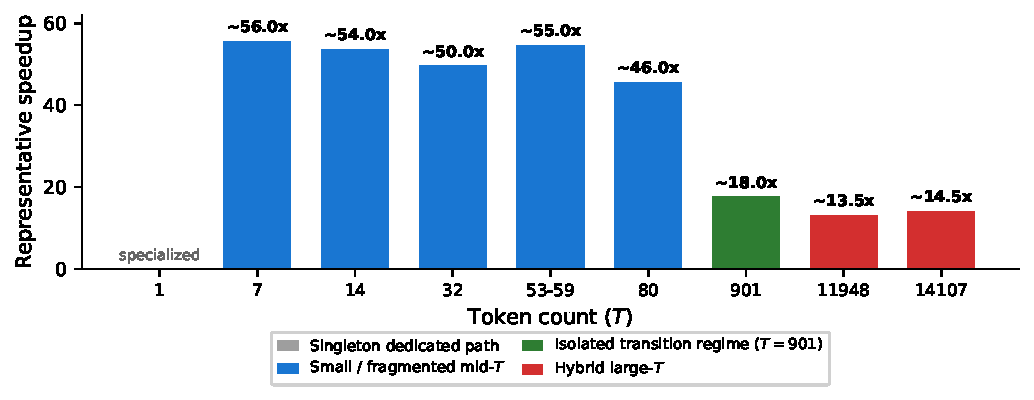
\includegraphics[width=0.95\linewidth]{figures/speedup_bar.pdf}
\end{center}
Small/mid-$T$ ($7$--$80$): ${\sim}46$--$56\times$ --- baseline launch overhead dominates, fused pipeline amortizes it.
Large-$T$ ($11{,}948$--$14{,}107$): ${\sim}13$--$15\times$ --- GEMM2 FP16 A-side prevents FP8 tensor core use.
The gap reflects the GEMM1$\to$GEMM2 bottleneck crossover: small-$T$ is GEMM1-bound (FP8 dot helps), large-$T$ is GEMM2-bound (FP16 A-side caps throughput).
\end{block}

\begin{block}{Kernel Time Breakdown \& TFLOPS}
\begin{minipage}[t]{0.48\linewidth}
\begin{center}
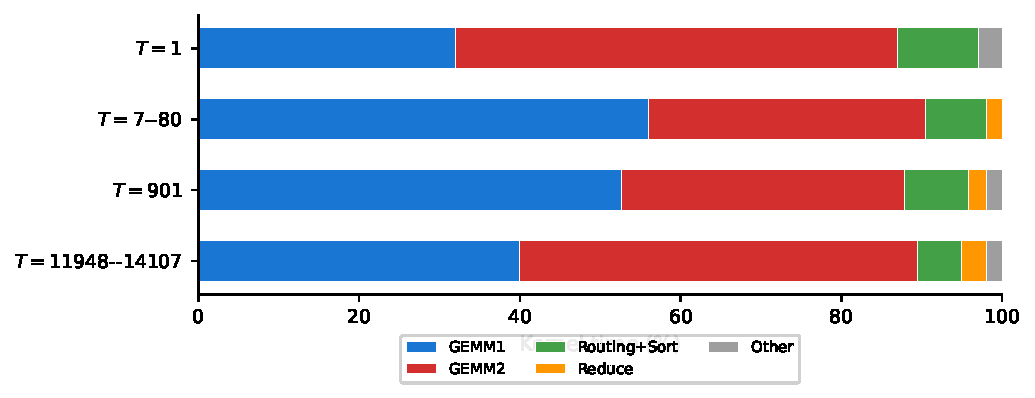
\includegraphics[width=\linewidth]{figures/time_breakdown.pdf}
\end{center}
\end{minipage}\hfill
\begin{minipage}[t]{0.48\linewidth}
\begin{center}
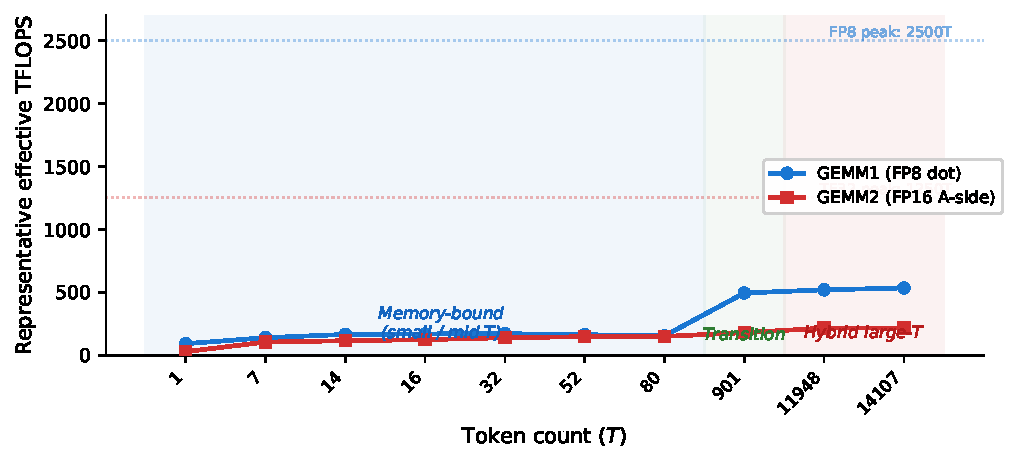
\includegraphics[width=\linewidth]{figures/tflops_efficiency.pdf}
\end{center}
\end{minipage}
\vspace{2pt}

\textbf{Small $T$:} GEMM1 dominates; expert weights repeatedly loaded for very few routed rows, with substantial padding waste.\\
\textbf{Large $T$:} GEMM2 becomes the main bottleneck; CuTe improves the grouped-GEMM core for the largest traces.\\
\textbf{CPU overhead:} Routing + sorting consumes ${\sim}600\,\mu$s (56--73\% wall time), but CUPTI scoring excludes it entirely.
\end{block}

\begin{block}{Optimization Timeline (23 Rounds)}
\begin{center}
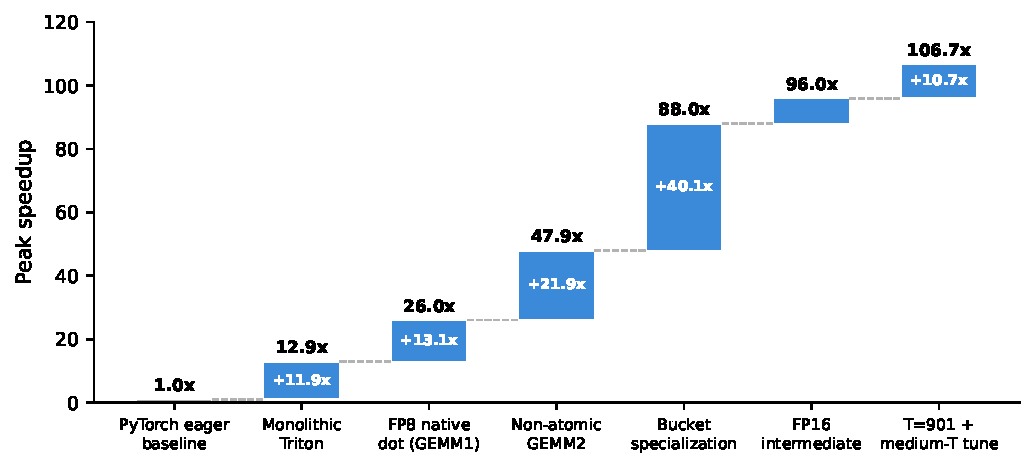
\includegraphics[width=0.95\linewidth]{figures/optimization_timeline.pdf}
\end{center}
Largest jumps: eliminating per-expert launches, FP8-dot/non-atomic GEMM2 backbone, workload-aware specialization.
Later gains are smaller but cumulative: compiler hints, deeper GEMM2 pipelining, bf16 expert\_out, exact large-$T$ dispatch, CuTe hybrid, and tight mid-$T$ BLOCK\_M tuning.
Rounds 11--15 explored persistent kernels, TMA, warp specialization, fused reduce --- all regressed or crashed.
\end{block}

\end{minipage}
\end{minipage}%
\hspace{\colsep}%
\begin{minipage}[t]{0.225\textwidth}
\begin{minipage}[t][\colheight][t]{\textwidth}

\begin{block}{Negative Results (8 Failed Attempts)}
\small
\begin{tabular}{@{}p{0.28\linewidth}p{0.12\linewidth}p{0.50\linewidth}@{}}
\toprule
\textbf{Approach} & \textbf{Result} & \textbf{Root Cause} \\
\midrule
FP8 Inter. & 0/19 & 3-bit mantissa; SwiGLU $>$ fp8 max \\[2pt]
bf16 Inter. & 8/19 & Low mantissa + reg.\ pressure \\[2pt]
Persistent & $-$1\% & K=2048 too short for reuse \\[2pt]
TMA Desc. & $-$4\% & Setup $>$ 16 K-loop iters \\[2pt]
Warp Spec. & Crash & TTGIR lowering failure \\[2pt]
Fused Red. & $-$4.5\% & fp32 atomic $6\times$ bf16 BW \\[2pt]
CuTe mid-$T$ & No gain & Metadata/sync not amortized \\[2pt]
GEMM2 FP8 & 5/19 & fp16$\to$fp8 cast too lossy \\
\bottomrule
\end{tabular}
\normalsize
\vspace{4pt}

Two failure groups: lower-precision buffers break correctness; persistence, TMA, fusion, and mid-$T$ CuTe do not amortize setup for $K{=}2048$ (only 16 K-loop iterations).
\end{block}

\begin{block}{Key Takeaways}
\begin{enumerate}
\item \textbf{Understand scoring:} CUPTI GPU-only timing hides ${\sim}600\,\mu$s CPU overhead---don't optimize what isn't measured
\item \textbf{Precision $\ne$ spectrum:} FP16 passes 19/19 (+4.5\%); bf16 Intermediate fails 11/19; fp8 fails all---mantissa bits matter more than range
\item \textbf{A/B test everything:} $\pm$15\% per-workload noise demands same-session comparison ($>$2\% threshold)
\item \textbf{Profile first:} All 8 successful techniques identified via NCU profiling, not speculation
\item \textbf{Tolerance matters:} Contest $\text{atol}{=}1.0$ unlocks bf16 expert output ($+0.4\%$ mean) that fails strict $\text{atol}{=}0.01$
\end{enumerate}
\end{block}

\begin{block}{Future Work}
\begin{itemize}
\item Small-$T$ memory-boundedness: 5.6\% of FP8 peak at $T{=}7$ (expert weight cold misses)
\item L2 persistent cache and epsilon expert skipping: prototyped but disabled pending tuning
\item MXFP8 \texttt{tl.dot\_scaled}: matched\_ratio = 0.17--0.32 (shared exponents too coarse for GEMM2)
\item Workload-adaptive kernel switching for production MoE serving
\end{itemize}
\end{block}

\begin{block}{Measurement Noise}
Modal B200 shared instances exhibit ${\pm}2\%$ mean noise across 19 workloads, with ${\pm}15\%$ per-workload variance for small $T$ ($<$0.2\,ms kernels) and $<$1\% for large $T$ ($>$2\,ms). Cross-session drift reaches ${\pm}20{-}30\%$ from co-tenant GPU interference. Our methodology: same-session A/B comparison with 2\% mean threshold --- only optimizations exceeding this noise floor are retained. Over 23 rounds, this discipline rejected 8 approaches that initially appeared promising (see Negative Results). Contest tolerance ($\text{atol}{=}1.0$) enables bf16 expert output (abs errors up to ${\sim}600$K) that would fail strict validation ($\text{atol}{=}0.01$).
\end{block}

\begin{block}{References}
\small
[1] DeepSeek-AI, ``DeepSeek-V3 Technical Report,'' arXiv:2412.19437, 2024.\\
{[2]} Tillet et al., ``Triton: An Intermediate Language and Compiler for Tiled Neural Network Computations,'' MLSys 2019.\\
{[3]} Darvish Rouhani et al., ``Microscaling Data Formats for Deep Learning,'' arXiv:2310.10537, 2023.\\
{[4]} Ye et al., ``FlashInfer: Efficient and Customizable Attention Engine for LLM Inference Serving,'' arXiv:2501.01005, 2025.\\
{[5]} Kerr et al., ``CUTLASS: Fast Linear Algebra in CUDA C++,'' NVIDIA, 2017--2025.
\end{block}

\end{minipage}
\end{minipage}

% ---- FOOTER (pinned to bottom) ----
\vfill
\begin{beamercolorbox}[wd=\textwidth,sep=0.2cm]{block title}
\centering
{\small\color{white}\textbf{MLSys 2026 FlashInfer-Bench Challenge --- Track A} \qquad Jiayao Zhang ~\textbullet~ Jiaoliang Yu}
\end{beamercolorbox}
\vspace{-3.5mm}

\end{frame}
\end{document}
